 \section{Introduction}
  \label{Intro}
  This report describes the design and performance of a Pattern Recognition algorithm that is able to classify images of hand-written digits on bank cheques. It considers two cases:
  \begin{itemize}
  	\item \textbf{Case I: The system is trained only one time, and then used in the field.} This means a large amount of training data is available.
  	\item \textbf{Case II: The system is trained for each batch of cheques.} This means only a small amount of training data is available.
  \end{itemize}
Although Case II provides significantly less data than Case I (and this definitely has to be taken into account during the design of the classification system) it is worthy to note that both cases call for a supervised learning approach. \\
The available data will be extracted from the NIST-list, a large dataset containing labelled hand-written digits from 0 to 9. These images will be processed in order to make it easier to handle them. The loading of the list and processing of the images it contains is done in a separate function. \todo[]{even de titel van de m-file noemen (dus hoe de functie heet)} This function is descibed in detail in section \ref{sec:ImPros}. Implementing the pre-processing in this way enables the inclusion of the image-processing part of the algorithm in a later benchmark test. It also enables us to keep the pre-processing consistent across the two different cases.\\
\indent After the processing, two classifiers will be trained, one for each of the aforementioned cases. These classifiers will be stored as $w$, so that they too can be implemented in the benchmark test. The design of these classifiers is described in detail in section \ref{sec:ClasDes}. \\
\indent Finally, for both cases, the benchmark test will be conducted by calling \texttt{e = nist eval(filename,w,n)}. The error $e$ this function returns should be less than 5\% for case 1 and less than 25\% for case 2. An overview of the handling of the data can be seen in figure \ref{fig:process_flow}.
\begin{figure}[H]
	\centering
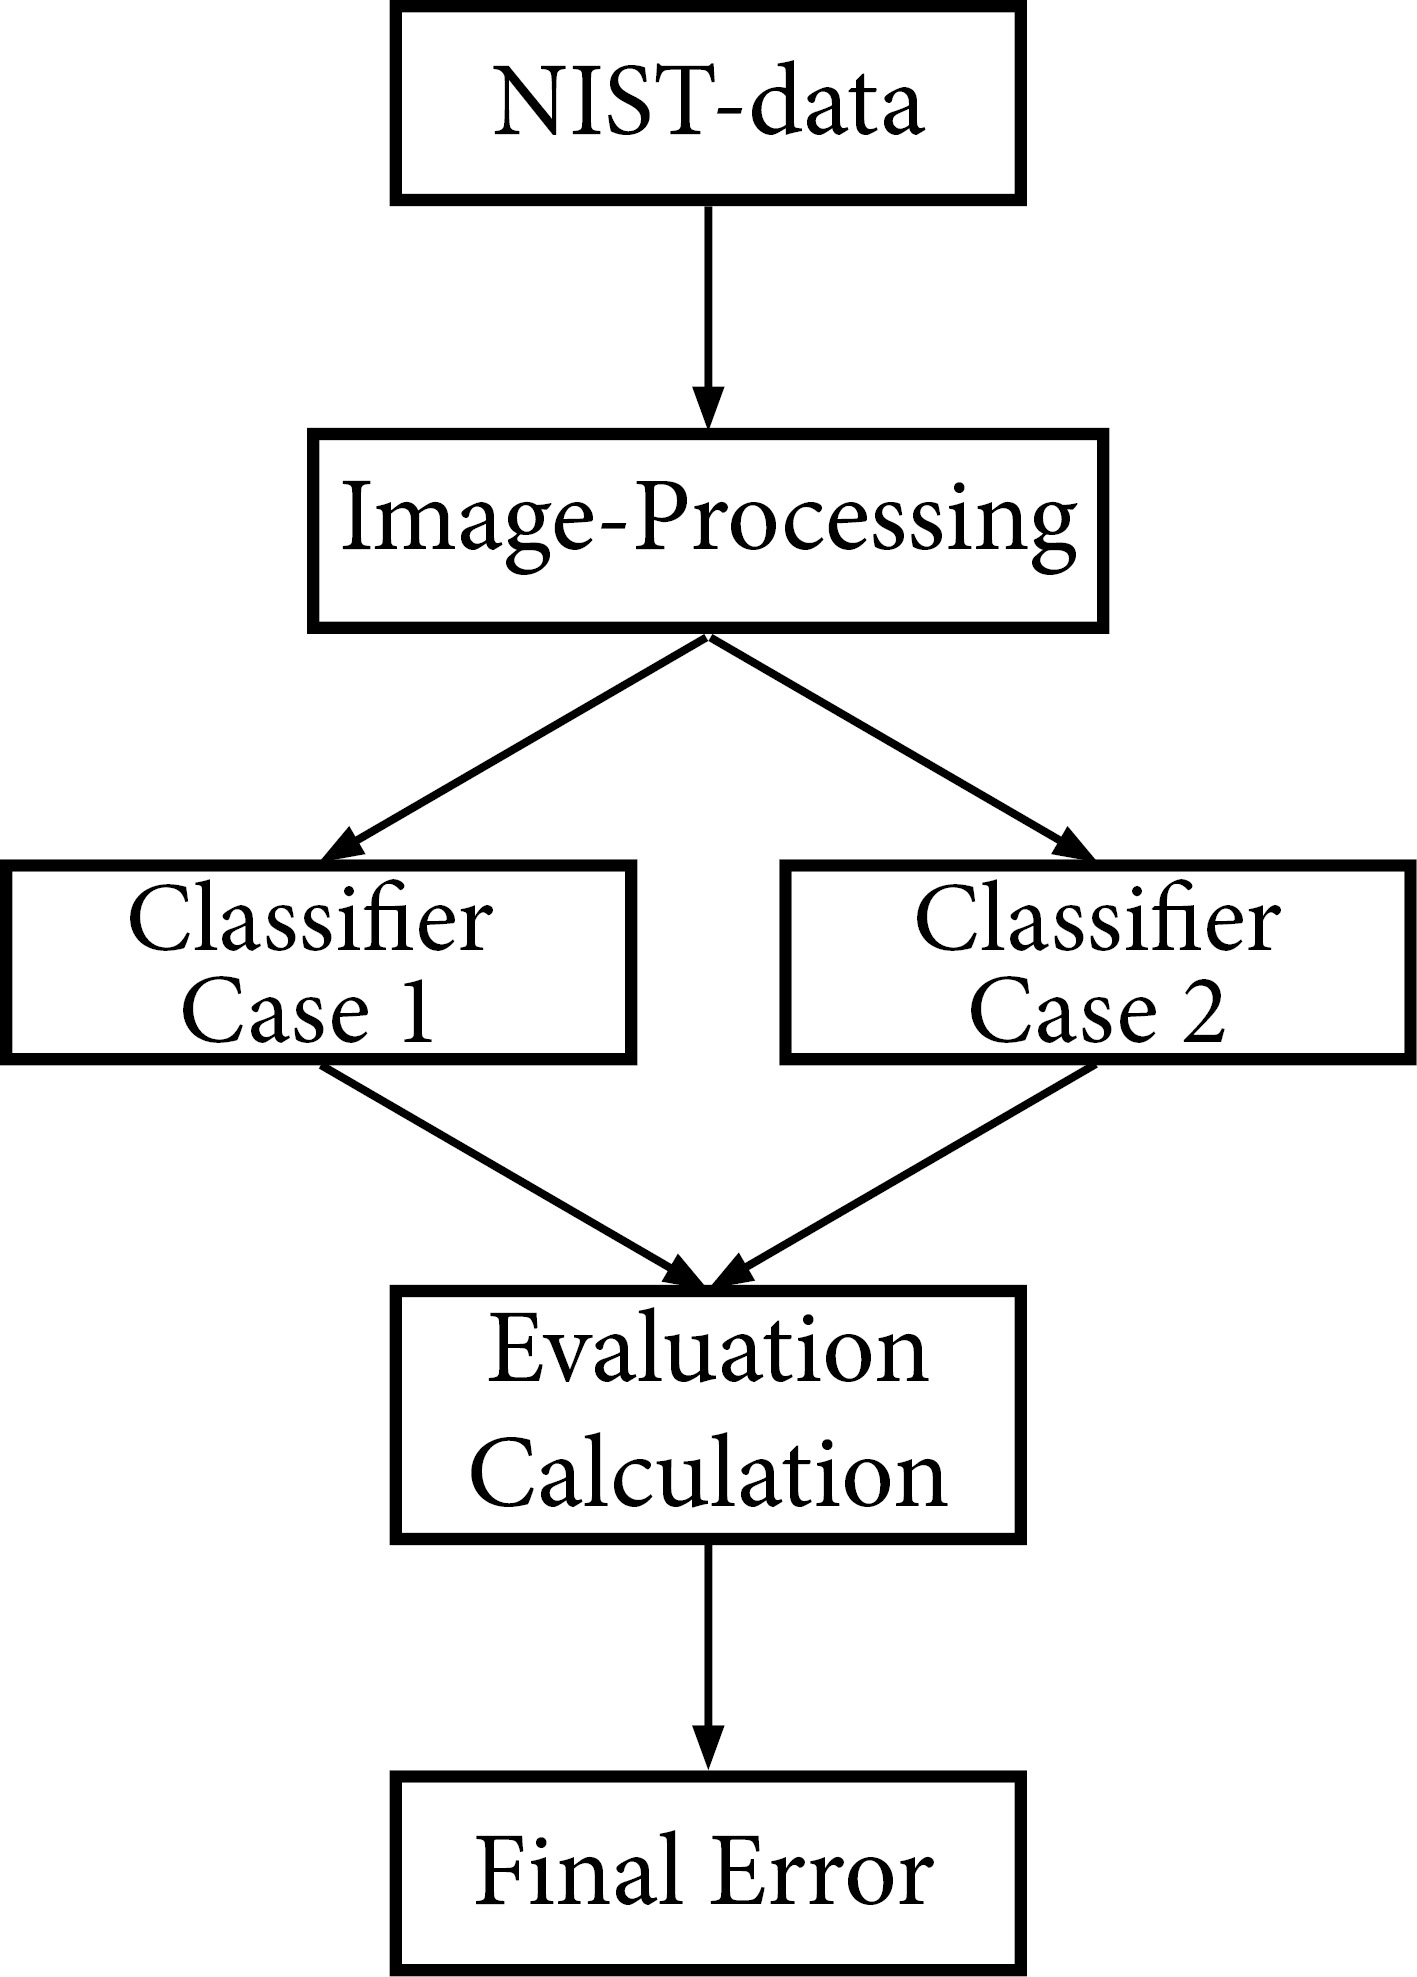
\includegraphics[scale=0.65]{images/Process_Flow.jpg}
\caption{Process of classification of the NIST-data for the two cases.}
\label{fig:process_flow}
\end{figure}